% TODO: write appendices
\appendix
\chapter{Hardware modification enabling serial communication}
\label{appendix:uard_pins}

Here we describe the steps necessary to enable serial communication
between the watch and the PC. On the PC side, serial port will be
emulated through USB, by the same USB debug dongle that is used to
flash program images on the watch. It is a very convenient solution.

We'll start by looking and the USB dongle. Figure
\ref{fig:chronos_dongle_pins} shows the function of the dongle pins.
\begin{figure}[h]
  \centering
  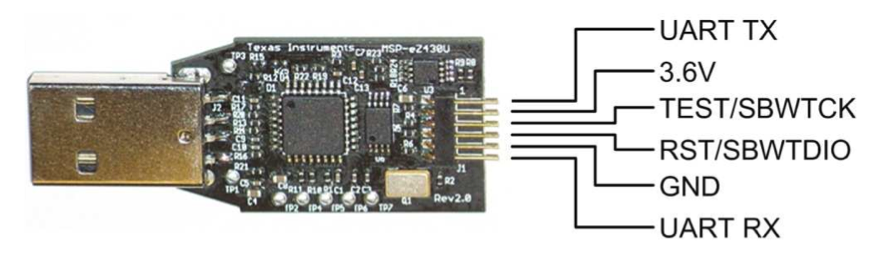
\includegraphics[width=0.7\textwidth]{img/chronos_dongle_pins.png}
  \caption{Pin functions of the USB debug dongle (Courtesy Texas Instruments)}
  \label{fig:chronos_dongle_pins}
\end{figure}
Ones labeled \emph{UART TX} and \emph{UART RX} are responsible for
serial communication. However if you look at chronos watch schematics,
you'll see that these pins remain unconnected in the watch. Relevant
snippet is shown in figure \ref{fig:chronos_unonnected_uart}
\footnote{Schematics are published in \cite{eZ430Chronos} and also
shown in appendix \ref{appendix:watch_schematics} for quick
reference.}.
\begin{figure}[h]
  \centering
  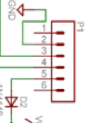
\includegraphics[width=0.15\textwidth]{img/chronos_unonnected_uart.png}
  \caption{Unconnected UART pins on the watch (Courtesy Texas Instruments)}
  \label{fig:chronos_unonnected_uart}
\end{figure}
This is exactly what needs to be fixed. Fortunately the MCU is capable
of dynamic port remapping. This means that these UART pins may be
connected to any two IO pins and software can handle rest of the
configuration.

% TODO(horban): dokoncz to


%------------------------------------------------------------------------------

\appendix
\chapter{Chronos watch schematics}
\label{appendix:watch_schematics}

\begin{figure}[h]
  \centering
  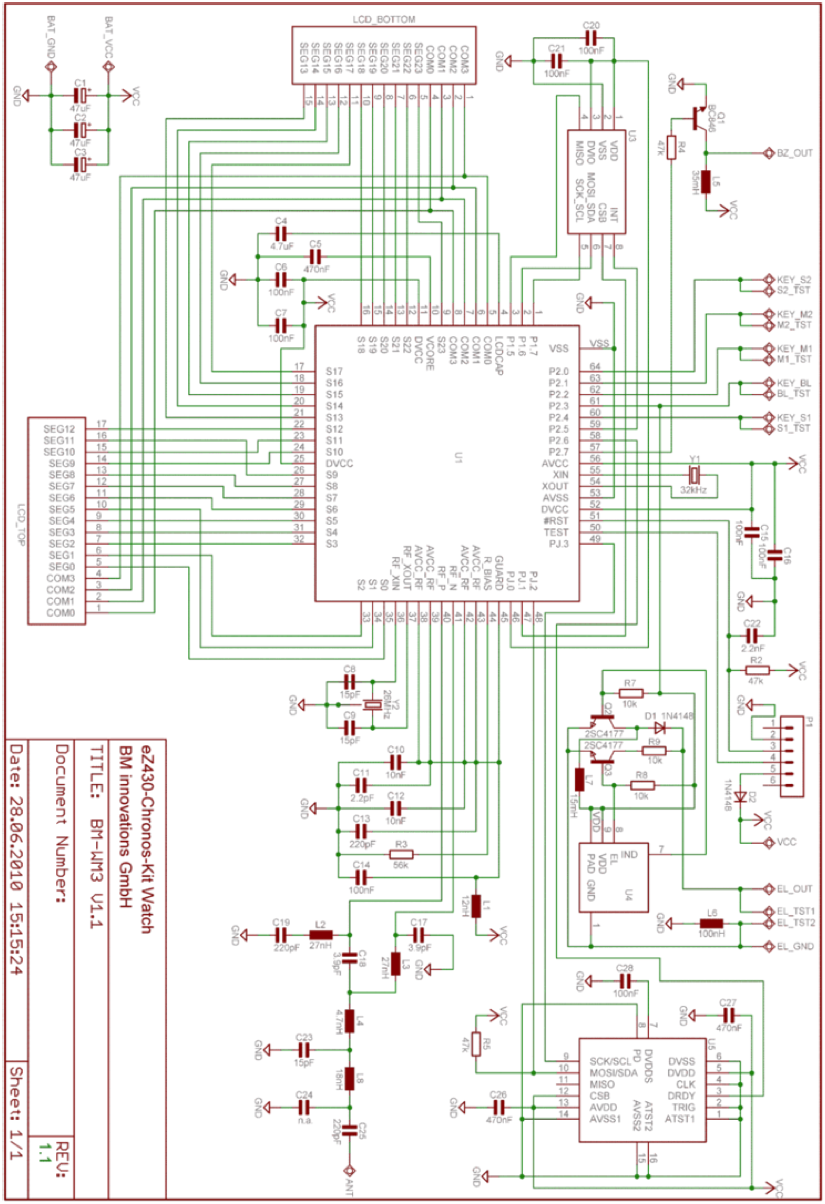
\includegraphics[width=1.0\textwidth]{img/watch_schematics.png}
  \caption{(Courtesy Texas Instruments)}
\end{figure}


% Vim settings:
% vim: set textwidth=70:
% vim: set fo+=t:
